
\section{Evaluating ActiveRecord Safety}
\label{sec:evaluation}

In the previous section, we identified two classes of commonly used
invariants that were not invariant confluent and therefore sensitive
to concurrent execution: uniqueness constraints and associations under
concurrent deletion and insertion. In this section, we evaluate
how well Active Record actually guards against these class of
violations. 

\subsection{Uniqueness Constraints and Isolation}

To begin, we consider Rails's uniqueness validations: 12.7\% of the
built-in validations we encountered.

When a Model field is declared with a \texttt{:validates\_uniqueness}
annotation, any instance of that model is checked against all other
models in the database to ensure uniqueness. Rails accomplishes this
by issuing a \texttt{SELECT WHERE} query in SQL and, if no such record
is found, Rails updates the instance state in the database.

While this user-level uniqueness validation runs within a transaction,
the exact isolation level of the transaction affects its
correctness. For correct execution, the \texttt{SELECT} query must
effectively attain a predicate lock on the validated column for the
duration of the transaction. This behavior \textit{is} supported under
serializable isolation. However, under Read Committed or Repeatable
Read isolation, no such mutual exclusion will be performed, leading to
potential inconsistency.\footnote{Using \texttt{SELECT FOR UPDATE}
  under these weaker models would be safe, but Rails does not
  implement its predicate-based lookups as such (i.e., it instead opts
  for a simple \texttt{SELECT}).}  Moreover, under Snapshot Isolation,
insertions to different records will similarly result in
inconsistency.\footnote{The first reference to the potential integrity
  violations resulting from this implementation in the Rails code that
  we are aware of dates to December 2007, in Rails v.2.0.0
  (\url{https://github.com/rails/rails/commit/c01c28c3047bbf0be2861c7ae1146723cf4ff7a9})
  In September 2008, another user added additional discussion
  (\url{https://github.com/rails/rails/commit/adacd9451877d3c195da7f1935353b1cb3fed368}),
  noting that ``this could even happen if you use transactions with
  the 'serializable' isolation level.'' Without reading too closely,
  the use of ``'serializable''' possibly suggests familiarity with the
  common, erroneous labeling of Snapshot Isolation as ``serializable''
  (as in Oracle 12c documentation and PostgreSQL documentation prior
  to the introduction of SSI in version 9.1.1 in September 2011.)\label{fn:si-rails}. }
Thus, unless the database is configured for serializable isolation,
inconsistency may result and the feral validation will fail.

As we have discussed, MySQL and PostgreSQL each support serializable
isolation but default to weaker isolation. Notably, in our
investigation, we discovered a bug in PostgreSQL's implementation of
Serializable Snapshot Isolation that allowed duplicate records to be
created under serializable isolation when running a set of
transactions derived from the Rails primary key validator. We omit
further details due to double-blind reviewing requirements but as of
October 2014 (PostgreSQL 9.3.5) have confirmed this behavior with the
core PostgreSQL developers who are currently working on a patch. Thus,
any discussion of weak isolation levels aside, PostgreSQL's
implementation of serializablility is not actually sufficient to
provide correct behavior for the above uniqueness validations. We note
that ``serializable'' databases such as Oracle 13g that actually
provide Snapshot Isolation will similarly fall prey to duplicate
validations.

Interestingly, the Rails documentation actually warns that duplicate
records may be inserted even despite uniqueness
validations~\cite{rails-guide}. However, despite the existence of
patches that remedy this behavior by the use of an in-database
constraint and/or index, Rails provides this incorrect behavior out of
the box.\footnote{\url{https://github.com/rails/rails/issues/645}} To
quote one Rails issue: ``this is not a bug but documented and inherent
behavior of
validates\_uniqueness\_of''.\footnote{\url{https://github.com/rails/rails/issues/13234#issuecomment-30092363}} In an apparent departure from the Rails's stated philosophy, a
core committer follows up, noting that ``the only way to handle this
properly is at the database layer with a unique constraint on the
column.'' We further discuss this mismatch between framework and database
guarantees in Section~\ref{sec:discussion}

\minihead{Understanding validation behavior} Given that entirely feral
mechanisms can introduce duplicates, how many duplicates can be
introduced? Once a record is written, any later validations will
observe it via \texttt{SELECT} calls. However, \textit{while} a record
is being validated, any number of concurrent validations can
(un)safely proceed. In practice, the number of concurrent validations
is dependent on the Rails environment. In a Rails deployment
permitting $P$ concurrent validations (e.g., a single-threaded,
multi-process environment with $P$ processes), each value in the
domain of the uniqueness validation can be inserted no more than $P$
times. Thus, validations---at least theoretically---reduce the
worst-case number of duplicate records for each unique value in the
column.

\subsection{Quantifying Uniqueness Anomalies}

Given that feral uniqueness validations are $i.)$ acknowledged to be
broken (at least under non-serializable isolation), $ii.)$ have a
work-around by correctly declaring them within the database, yet
$iii.)$ are widely used, we sought to understand their costs and
benefits in an actual production environment. Accordingly, we wrote
and deployed a custom Rails 4 application that exercised uniqueness
validations and observed its behavior under various workloads.

\minihead{Experimental setup} We developed a Rails 4 application that
performed insertions to a non-indexed string column and compared the
degree of violations both with and without a uniqueness validator. We
deployed this application across two Amazon EC2 \texttt{m2.4xlarge}
instances, offering 68.4 GB RAM, 8 CPU cores, and 1680GB local
storage, running Ubuntu 14.04 LTS. On one instance, we deployed our
application, using nginx 1.6.2 as a web frontend proxied to a set of
Unicorn 4.8.3 workers. That is, nginx acts as a HTTP frontend and
forwards incoming requests to a variably sized pool of Rails VMs
(managed by Unicorn, in a multi-process single-threaded concurrency
model) that, in effect, \texttt{epoll} on a shared Linux file
descriptor. On the other EC2 instance, we deployed PostgreSQL 9.3.5
and configured it to run on the instance local storage. We used a
third EC2 instance to direct traffic to the front-end instance and
drive load. We plot the average and standard deviation of three runs
per experiment.

\minihead{Stress test} We began our study by issuing a simple stress
test that executed a number of concurrent insertion requests against a
variable number of Unicorn workers. We repeatedly issued a set of 64
concurrent model creation (SQL insertion) requests, each with the same
validated key (e.g., all with field \texttt{key} set to value 1)
against the Rails application. Across an increasing number of Unicorn
workers, we repeated this set of requests 100 times (blocking
in-between rounds to ensure that each round is, in fact, a concurrent
set of requests), changing the validated key each round.

Figure~\ref{fig:pk-stress} shows the results. With no validation, all
concurrent requests succeed, resulting in 6300 duplicate records (100
rounds of 64-1 duplicate keys). With validations enabled, the number
of violations depends on the degree of concurrency allowed by
Unicorn. With only one process, Unicorn performs the validations
serially, resulting in no duplicates. However, with two processes,
Unicorn processes begin to race, resulting in 70 duplicate records
spread across 70 keys. With three processes, Unicorn produces 249
duplicate records across all 100 keys. The number of duplicates
increases with the number of processes, maximizing at 16 worker
processes. With additional processes, duplicates slightly decrease,
which we attribute to thrashing between processes and within
PostgreSQL (given that each instance has only 8 cores). Nevertheless,
using validations, the microbenchmark duplicate count remains below
700---nearly an order-of-magnitude fewer duplicates than without using
validations. Therefore, even though these validations are, in fact,
incorrectly implemented, they still result in fewer
anomalies. However, with a unique index declared on the \texttt{key}
column, we observed no duplicates, as expected.

\begin{figure}
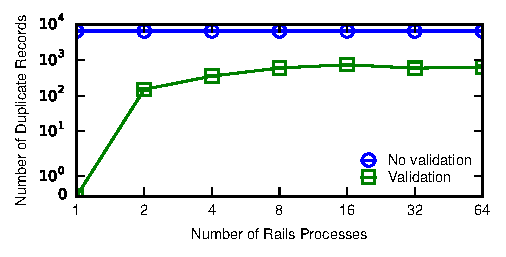
\includegraphics[width=\columnwidth]{figs/pk_stress_violations.pdf}
\caption{Uniqueness stress results.}
\label{fig:pk-stress}
\end{figure} 

\minihead{Actual workloads} The preceding experiment stressed a
particularly high-contention workload---in effect, a worst case
workload for uniqueness validations. In practice, such a workload is
likely rare.\footnote{In fact, it was in the above workload that we
  encountered the non-serializable PostgreSQL behavior under
  serializable isolation. Under serializable isolation, the number of
  anomlies is reduced compared to the number under Read Committed
  isolation (as we report here), but we still detected duplicate
  record creation. We confirmed this non-serializable behavior via
  subsequent implementations of this parallel
  predicate-read-then-conditionally-insert workload in both Python and
  PostgreSQL PL/pgSQL stored procedures.} Accordingly, we set up
another workload meant to capture a less pathological access
pattern. We ran another insert-only workload, with key choice
distributed among a fixed set of keys. By varying the distribution and
number of keys, we were able to both capture more realistic workloads
and also control the amount of contention in the workload. As a basis
for comparison, we ran four different distributions. First, we
considered uniform key access. Second, we used YCSB's
Zipfian-distributed accesses from
\texttt{workloada}~\cite{ycsb}. Third and fourth, we used the item
distribution access from Facebook's LinkBench workload, which captures
MySQL record access when serving Facebook's social
graph~\cite{linkbench}. Specifically, we used---separately---the
insert and update traffic from this benchmark.

For each trial in this workload, we used 64 concurrent clients
independently issuing a set of 100 requests each, with a fixed number
of 64 Unicorn workers per process. 

Figure~\ref{fig:pk-workload} illustrates the number of duplicate
records observed under each of these workloads. As we increase the
number of possible keys, there are two opposing effects. With
more keys, the probability of any two operations colliding
decreases. However, recall that, once a key is written, all subsequent
validators can read it. Therefore, increasing the number of keys
increases the total number of possible races that might
occur. Therefore, while the uniform workload observes an average of
2.33 duplicate records with only one possible key, it observes an average of 26
duplicate keys with 1000 possible keys. Nevertheless, with 1 million possible
keys, we do not observe any duplicate records.

The actual ``production'' workloads exhibit different trends. In
general, YCSB is an extremely high contention workload, with a Zipfian
constant of 0.99, resulting in one very hot key. This decreases the
beneficial effect of increasing the number of keys in the
database. However, LinkBench is less contentious and decreases more
rapidly with increased numbers of keys.

\begin{figure}
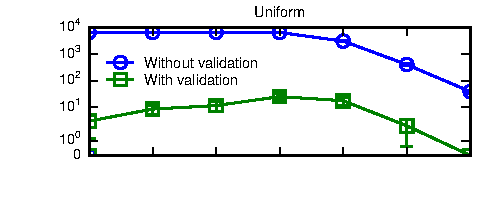
\includegraphics[width=\columnwidth]{figs/pk-workload-uniform-violations.pdf}\vspace{-2em}
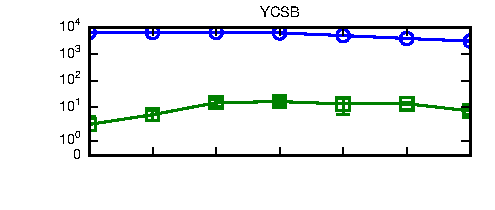
\includegraphics[width=\columnwidth]{figs/pk-workload-ycsb-violations.pdf}\vspace{-2em}
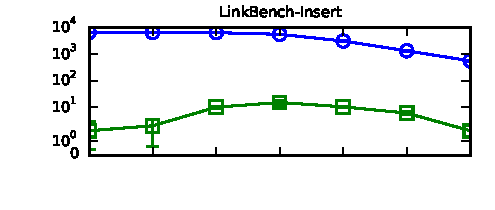
\includegraphics[width=\columnwidth]{figs/pk-workload-linkbench-ins-violations.pdf}\vspace{-2em}
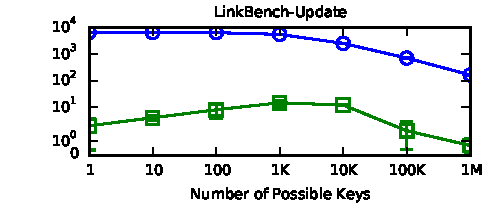
\includegraphics[width=\columnwidth]{figs/pk-workload-linkbench-upd-violations.pdf}\vspace{-1em}
\caption{Uniqueness workload results.}
\label{fig:pk-workload}
\end{figure}

\subsection{Associations}

We repeated another set of experiments to test association behavior
under insertions and deletions. Using the same Unicorn and PostgreSQL
deployment, we configured another application to test whether or not
Rails validations would defend against dangling entries.

As a basic stress test, we consider an application with two models:
Users and Departments. We configure a one-to-many relationship: each
user \texttt{belongs\_to} a department, and each department
\texttt{has\_many} user. In the workload, we initialize the database
by creating 100 departments with no users. Subsequently, for each
department in the database, we issue a single request to delete the
department along with 64 concurrent requests to insert users in that
department. To correctly preserve the one-to-many relationship, the
database should either reject the deletion operation or perform a
cascading deletion of the department and any users (while rejecting any
future user creation requests for that department). We can quantify
the degree of inconsistency by counting the number of users left in
the database who have no corresponding department.

With associations declared in Rails, the Rails process performing the
deletion will attempt a cascading delete of users upon department
deletion. However, this cascade is performed, again, ferally---at the
application level. Thus, under non-serializable isolation, any user creation
events that are processed while the search for Users to delete is
underway will result in Users without departments.

Figure~\ref{fig:fk-stress} shows the number of dangling Users as a
function of Rails worker processes. With no constraints declared to
Rails or to the database, all User creations succeed, resulting in
6400 dangling Users. With constraints declared in Rails (via a mix of
validation and association), the degree of inconsistency depends on
the degree of parallelism. Under the worst case, with 64 concurrent
processes, the validations are almost worthless to prevent
inconsistency. In contrast, when we declare a foreign key constraint
within the database, we observe no inconsistency.

\begin{figure}
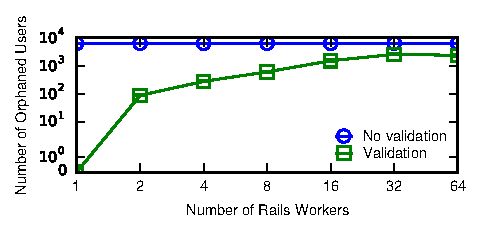
\includegraphics[width=\columnwidth]{figs/fk-stress-violations.pdf}\vspace{-1em}
\caption{Foreign key stress results.}
\label{fig:fk-stress}
\end{figure}

The above stress test shows that inconsistency due to feral
concurrency control occurs only during times of contention---parallel
deletions and insertions. We subsequently varied the degree of
contention within the workload. We configured the same application and
performed a set of insertions and deletions, but spread across a
greater number of keys and at random. A set of 64 processes
concurrently each issued 100 User creation and Department deletion requests (at
a ratio of 10 to 1) to a set of randomly-selected keys (again at a ratio of 10
Users to each Department). By varying the number of Users and
Departments, we were able to control the amount of contention within
the workload. Under this workload, inconsistency resulted only when a
Department deletion proceeded concurrently with a User creation event
and the feral cascading deletion ``missed'' the User creation.

Figure~\ref{fig:fk-workload} shows the results. As the number of
Departments increases, we observe two trends. First, with only one
Department, there is again less chance of inconsistency: all
operations contend on the same data item, so the total number of
inconsistent data is limited by racing deletions. However, with
increasing Departments, the number of inconsistent records decreases
linearly with the number of records.

\begin{figure}
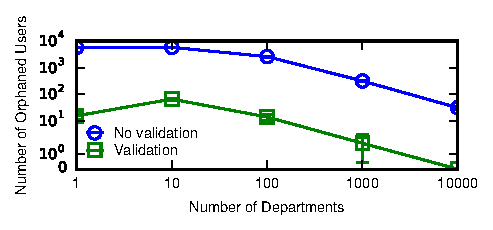
\includegraphics[width=\columnwidth]{figs/fk-workload-violations.pdf}\vspace{-1em}
\caption{Foreign key workload results.}
\label{fig:fk-workload}
\end{figure}

\subsection{Discussion}

The preceding experiments demonstrate that, indeed, Active Record is
unsafe as deployed by default. Validations are susceptible to data
corruption due to sensitivity to weak isolation anomalies. Moreover,
in PostgreSQL, current transaction support is insufficient to prevent
all anomalies.

This raises the question: why declare validations at all? As we
observe, validations protect against \textit{some} data
corruption. First, they correctly guard against
non-concurrency-related anomalies such as data entry or input
errors. For example, if a user attempts to reserve a username that was
previously chosen, a validation would succeed. The failures we observe
here are solely due to concurrent execution. Without concurrent
execution, validations are correct. Second, validations
\textit{do} reduce the incidence---if not the degree---of
inconsistency. Empirically, even under worst-case workloads, these
validations result in order-of-magnitude reductions in
inconsistency. Under less pathological workloads, they may reduce it
almost entirely. It is possible that, in fact, the degree of
concurrency and data contention within Rails-backed applications
simply does not lead to these concurrency races---that, in some sense,
validations are ``good enough'' for many applications.

Nevertheless, Rails's feral mechanisms are a poor substitute for their
respective database counterparts in both cases. We re-examine the Rails community's
reluctance to embrace these mechanisms in Section~\ref{sec:discussion}.

